\documentclass{turabian-researchpaper}

\usepackage[english]{babel}
\usepackage[utf8]{inputenc}
\usepackage{csquotes} 
\usepackage{multicol}
\usepackage[T1]{fontenc}    % use 8-bit T1 fonts
\usepackage{hyperref}       % hyperlinks
\usepackage{url}            % simple URL typesetting
\usepackage{booktabs}       % professional-quality tables
\usepackage{amsfonts}       % blackboard math symbols
\usepackage{nicefrac}       % compact symbols for 1/2, etc.
\usepackage{microtype}      % microtypography
\usepackage{lipsum}
\usepackage{graphicx}
\graphicspath{ {./images/} }
\usepackage{dsfont} 
\usepackage{amsmath}
\usepackage{amssymb}
\usepackage{amsthm} 
\newtheorem*{conjecture*}{Conjecture}
\newtheorem*{theorem*}{Theorem} 
\newtheorem{case}{Case} 
\newtheorem{case*}{Case} 
\newtheorem*{subcase*}{Subcase}
\usepackage{graphicx} 
\usepackage{float} 
\usepackage{subcaption}
%\usepackage{natbib} 
\usepackage{cleveref}
%\usepackage{biblatex-chicago}
%\addbibresource{references[1].bib}
\usepackage{natbib}
\usepackage{tikz} 
\usepackage{enumitem}
\usetikzlibrary{calc} 
\usepackage{pdfpages}

\title{Exploring a relationship between Linear Algebra and Physics: Torque and Cross Product}
\author{Siyabulela Tyaliti \\
  School of Health, Science, and Technology \\
  Bachelor of Science in Mathematics \\ 
  Cornerstone University \\
  Grand Rapids, MI 49525 \\
  \texttt{School email: \href{mailto:siyabulela.tyaliti@cornerstone.edu} {siyabulela.tyaliti@cornerstone.edu}} \\ 
  \texttt{Personal email: \href{mailto:siyabulelatyaliti@gmail.com}{siyabulelatyaliti@gmail.com}} \\ 
  %% \AND
  %% Coauthor \\
  %% Affiliation \\
  %% Address \\
  %% \texttt{email} \\
  %% \And
  %% Coauthor \\
  %% Affiliation \\
  %% Address \\
  %% \texttt{email} \\
  %% \And
  %% Coauthor \\
  %% Affiliation \\
  %% Address \\
  %% \texttt{email} \\} 
  }
  
\date{November 30, 2024} 

\begin{document}

\maketitle

\begin{abstract}
    In this paper I explored the an idea that relates an idea from physics and an idea from linear algebra. The goal of the research I worked on for this paper was for me to learn something new about physics or linear algebra, as I studied some facets of the relationships between physics and linear algebra. Over the course of my research for this paper, I worked on a problem that involved finding the torque on an object using the cross product. In the process of my research for this paper, I also got to learn something new within the subject of physics, I learned a lot about rotational motion and how we can apply the laws of kinematics to rotational motion in order for us to study how objects move as they rotate in the real world or in our everyday lives. 
\end{abstract}

\section{Introduction} 
The reason that we study physics is because physics allows us to figure out how the world works (and even how the universe works in some case), and it helps us figure out our place in the world around us (\cite{CrashCoursePhysicsPreview2024}). The reason that we study linear algebra is because linear algebra allows us to study the four fundamental vector subspaces (the row space, column space, null space, and the left null space) and what they they tell us about a matrix (\cite{TheBigPictureOfLinearAlgebra2024}). Over the course of my research in preparation to write this paper, I worked on a problem that allowed me to relate a concept from Linear Algebra with a concept from Physics. 

\section{Goal of the research in this paper} 

The goal of the research I did as I was working on this paper was for me to relate a concept from Linear Algebra with a concept from Physics through taking something I had learned from Linear Algebra and apply it to Physics, or take a concept from Physics and look at the theory behind the Mathematics applied in the Physics concept. The goal of the research was for me to learn something I had not learned before either in Physics or in Linear Algebra, while relating the two subjects.   

\subsection{Discussion of Methodology} 

Over the course of my research in preparation to write this paper, I decided to learn something I had not learned before in Physics and I solved a problem that applied a concept from Linear Algebra to Physics. I spent time studying \href{https://openstax.org/books/university-physics-volume-1/pages/10-introduction}{Chapter 10 from University Physics (openstax) Volume 1}. When I took the class in Physics I with Dr. Keller, the last chapter we covered was chapter 9 which was on collisions and linear momentum. Chapter 10 in the Physics textbook covered Fixed-Axis Rotation (which deals with rotational motion around a fixed axis of rotation, or basically kinematics, but for rotational motion around a fixed point).  

\subsubsection{relating linear algebra and physics} 

As I was studying chapter 10 from the Physics textbook, one of the concepts that I encountered was the concept of torque. One of the things I further learned about was the fact that we use the cross product to compute the magnitude of the torque vector. The idea of the cross product comes from studying vectors in linear algebra. 

\section{Concepts fundamental to the problem I solved} 

\subsection{Cross Product} 

The cross product of two vectors \(a\) and \(b\) is computed by using the formula \(a \times b = \lvert a \rvert \lvert b \rvert sin{\theta}\) \cite{CrossProductsUdemyNOTESKristaKingMath2024}. The cross product allows us to find how far apart two vectors are from each other \cite{DotandCrossProductsasOppositeIdeasUdemyNOTESKristaKingMath2024}. When we model this idea geometrically,   we see that you will have two vectors \(a\) and \(b\) that are some angle \(theta\) apart. We will also see that the two vectors are both perpendicular to some normal vector (some vector that is perpendicular to every vector in some vector space (the normal vector is usually perpendicular to some plane formed by some vector space))  

\subsection{Torque} 

Torque is defined as the force that is applied to objects when they move in rotational motion. The magnitude of the torque vector is calculated using the formula \(\left\lvert r \times F \right\rvert = \left\lvert \overrightarrow{r} \right\rvert \left\lvert \overrightarrow{F} \right\rvert\ sin{\theta}\) \cite[p.$\Tilde{496}$]{UniversityPhysicsVolumeONE2024}. The magnitude of the torque vector is largely dependent on the magnitude of the lever arm (represented by the displacement vector). Torque is a vector quantity and a vector quantity has both a magnitude and a direction. To find the direction of the torque vector we use the right hand rule \cite[p.$\Tilde{496}$]{UniversityPhysicsVolumeONE2024}. Torque can either be positive or negative depending on whether the torque vector rotates clockwise or counterclockwise. When the torque vector rotates in a  counterclockwise direction, then torque is positive. When the torque vector rotates in a clockwise direction, then torque is negative. The direction of rotation of the torque vector can be determined using the right-hand rule. To determine the direction of rotation of the torque vector using the right hand rule, you point your thumb in the direction of the force vector, and you point the rest of your fingers (or your index finger) in the direction of the displacement vector. When you close your right hand, the direction that your thumb naturally points to determines the sign of the torque (when your thumb points towards you (or when it points into the page), the torque vector is negative; when your thumb points away from you (or when it points out of the page), the torque vector is positive). Also, when you close your right hand, the direction that the rest of your fingers (or your index finger) rotate towards determines the direction of rotation of the torque vector. If the rest of your fingers (or your index finger) rotate in a clockwise direction, then the torque vector rotates in a clockwise direction. If the rest of your fingers (or your index finger) rotate in a counterclockwise direction, then the torque vector rotates in a counterclockwise direction \cite{torquewikihow2024}. Another way in which we can relate torque from physics to linear algebra concepts is that we can see that the torque vector is also the normal vector perpendicular to both the force vector and the displacement vector \cite{torquekhanacademy2024}. We can see this shown in the figure below: 

\begin{figure}[H] 
    \centering
    \includegraphics[width=0.5\linewidth]{Screenshot 2024-12-06 150159.png}
    \caption{Torque vector as a normal vector}
    \label{fig:torq-norm}
\end{figure} 

And we know the idea of a normal vector since it is orthogonal to a plane in Linear Algebra. 

\section{The Problem I solved for my capstone research} 

Problem from \href{https://openstax.org/books/university-physics-volume-1/pages/10-6-torque}{Chapter 10 University Physics (openstax) Volume 1} \\
\vspace{0.1cm} 
Check your understanding 10.6 \\
\vspace{0.1cm}
A larger ocean-going ship runs aground near the coastline, similar to the fate of the Costa Concordia, and lies at an angle of \(10^\circ\). Salvage crews must apply a torque to the right in order to float the vessel for transport. A force of \(5.0 \times 10^5 N\) acting at a point \(A\) must be applied to right the ship. What is the torque about the point of contact with the ship and the ground?  

\begin{figure}[H] 
    \centering
      \begin{tikzpicture}
         \draw[->, thick, blue] (0,0) -- (2,5); 
          \fill[black] (2,5.1) node[above left]{ship} circle (0.1cm);
          \fill[blue] (1.5,2.5) node[black]{\(10m\)}; 
          \draw[->, thick, orange] (2,5.1) -- (4,5.1) node[black, below]{\(5 \times 10^5N\)};
          \draw[dashed, thick, red] (2,5.1) -- (2.7,7);  
          \draw[black, thick] (2.42,5.1) arc (0:60:0.5cm); 
          \fill[black] (2.56,5.6) node[black]{\(10^\circ\)}; 
      \end{tikzpicture}
    \caption{Free Body Diagram for the problem}
    \label{fig:Problem-FBD} 
\end{figure}

Magnitude of the torque force vector 
\begin{align*}
    \left\lvert \overrightarrow{\tau} \right\rvert &= \left\lvert \overrightarrow{r} \times \overrightarrow{F} \right\rvert \\ 
                                                   &= \left\lvert \overrightarrow{r} \right\rvert \left\lvert \overrightarrow{F} \right\rvert sin\theta \\ 
                                                   &= (10m)(5 \times 10^5N)sin(10^\circ) \\  
                                                   &= 868240.8883 N m \\
                                                   &= 8.682408883 \times 10^5 Nm \\
\end{align*} 

My additional questions (self-generated): \\ 

\begin{enumerate}[label=(\roman*)]
    \item Use the right-hand rule to find the direction of the torque vector, then state whether the torque force vector moves into the page or out of the page. (also describe the right-hand rule procedure). 
    \item Draw the torque force vector in a three-dimensional space and then use your answer to Question (i) to show the rotational direction of the torque in your diagram.  
    \item Give an interpretation of your answer in question (ii) in the context of this story problem. 
\end{enumerate}   

Answers to my additional questions: \\ 

(i)\underline{Direction of torque} \\

The torque vector points into the page, this means the torque vector rotates in a clockwise direction. \\ 

\underline{Right hand rule procedure} \\ 

I pointed my thumb to the direction of the force vector applied to the right (the force of \(5 \times 10^5N\). I pointed the rest of my fingers toward the direction of the displacement vector (the displacement \(10m\)), when I closed my right hand, my thumb naturally pointed into the page and the rest of my fingers rotated in a clockwise direction. \\ 

Side note: Before doing the right-hand rule, I moved the force vector from the head of the displacement vector (as seen from figure \ref{fig:Problem-FBD}) to the tail of the displacement vector. This can be seen in the diagram below: \\ 

\begin{figure}[H] 
    \centering
      \begin{tikzpicture}
         \draw[->, thick, blue] (0,0) -- (2,5); 
          \fill[black] (0,0) node[above left]{ship} circle (0.1cm);
          \fill[blue] (1.5,2.5) node[black]{\(10m\)}; 
          \draw[->, thick, orange] (0,0) -- (4,0) node[black, below]{\(5 \times 10^5N\)};  
          \draw[black, thick] (0.43,0) arc (0:60:0.5cm); 
          \fill[black] (0.57,0.5) node[black]{\(10^\circ\)}; 
      \end{tikzpicture}
    \caption{Free Body Diagram for the problem with an adjusted force vector} 
    \label{fig:Problem-FBD2} 
\end{figure}


(ii)  If we were to observe a three-dimensional projection of the free body diagram of the problem with the torque vector (on a two-dimensional surface (or a paper in this case)), we would see that we get the diagram below: \\ 

\begin{figure}[H] 
    \centering
      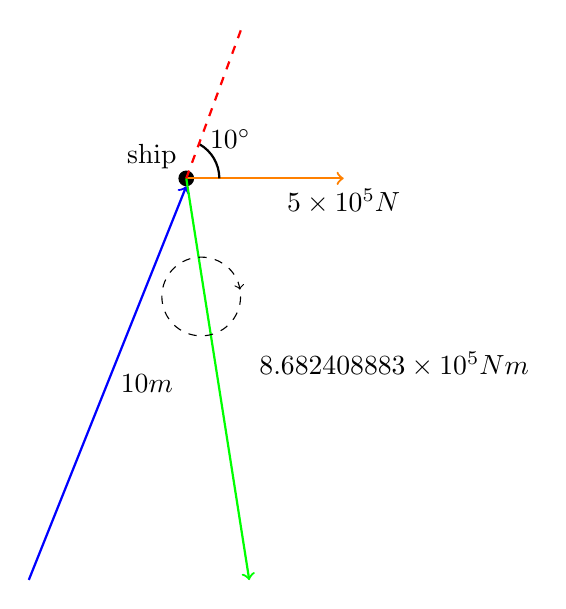
\begin{tikzpicture}
          \draw[->, thick, blue] (0,0,0) -- (2,5,0); 
          \fill[black] (2,5.1,0) node[above left]{ship} circle (0.1cm);
          \fill[blue] (1.5,2.5,0) node[black]{\(10m\)}; 
          \draw[->, thick, orange] (2,5.1,0) -- (4,5.1,0) node[black, below]{\(5 \times 10^5N\)};  
          \draw[black, thick] (2.42,5.1,0) arc (0:60:0.5cm); 
          \fill[black] (2.56,5.6,0) node[black]{\(10^\circ\)};
          \draw[->, thick, green] (2,5.1,0) -- (2.8,-0.001,0); 
          \draw[dashed, thick, red] (2,5.1,0) -- (2.7,7,0); 
          \fill[green] (1.9,-0.001,-7.12) node[black]{\(8.682408883 \times 10^5 Nm\)}; 
          \draw[->, dashed, black] (2.69,3.6,0) arc (0:-350:0.5cm); 
      \end{tikzpicture}
    \caption{ free body diagram of the problem with the torque vector}
    \label{fig:Problem-FBD3}
\end{figure} 

Side note: The blue vector represents the displacement, the orange vector represents the force to the right, and the green vector represents torque. Since the torque vector points into the page, the torque is therefore \(-8.682408883 \times 10^5 Nm\). \\ 

(iii) This means that to right the ship in order to float the vessel, the captain must steer the ship by rotating the steering gear in a clockwise direction with a torque of \(8.682408883 \times 10^5 Nm\). \\ 

\section*{A summary of everything else I learned from physics throughout my research} 

As I did my capstone research for this paper, through reading \href{https://openstax.org/books/university-physics-volume-1/pages/10-introduction}{Chapter 10 from University Physics (openstax) Volume 1}, I got to learn that before we can study torque, it is best for us to get some context about rotational variables. Variables such as the angular velocity which relates the angle of rotational motion to the radius (or distance between the object rotating and the center axis of rotation), angular acceleration which relates the angular velocity to the quantity of time. \\ 

When we think about kinematics and how that relates to rotational, we look at the laws of kinematics from translational motion and we replace the variables of linear translational motion in the laws of kinematics with the variable of rotational motion in the laws of kinematics. \\  

When we relate linear translational motion variables to rotational motion variables, we get the following table: \\
\vspace{0.5cm}

\begin{tabular}{|c|c|c|}
\hline
     & Linear  & Rotational \\
\hline
  Position   & \(x\)  & \(\theta\) \\
\hline
   Velocity  & $v = \frac{dx}{dt}$  & $\omega = \frac{d\theta}{dt}$  \\
\hline
  Acceleration   &  $a = \frac{dv}{dt}$ & $\alpha = \frac{d\omega}{dt}$  \\ 
  \hline 
\end{tabular} 
\vspace{0.5cm} 

And when we relate rotational kinematic equations to linear translational kinematics equations, we would obtain the following table: \\ 
\vspace{0.5cm} 

\begin{tabular}{|c|c|}
\hline
   Rotational  & Translational \\
\hline     
    $\theta_{f} = \theta_{0} + \overline{\omega}t$ & $x_{f} = x_{0} + \overline{v}t$ \\
\hline
   $\omega_{f} = \omega_{0} + {\alpha}t$ & $v_{f} = v_{0} + {a}t$ \\
\hline
 $\theta_{f} = \theta_{0} + \omega_{0}t +{\frac{1}{2}}{\alpha}t^2$   &  $x_{f} = x_{0} + v_{0}t +{\frac{1}{2}}{a}t^2$ \\
\hline
   ${\omega_{f}}^2 = {\omega_{0}}^2 + 2{\alpha}(\Delta\theta)$ & ${v_{f}}^2 = {v_{0}}^2 + 2{a}(\Delta{x})$ \\
\hline
\end{tabular}
\vspace{0.5cm} 

I also learned about rotational kinetic energy, the concept of rotational kinetic energy is basically the rotational counterpart of the concept and formula that we use when we calculate kinetic energy with respect to translational motion. In order for us to be able to calculate the rotational kinetic energy of an object as it rotates, we also need to know the moment of inertia across the path of the rotating object. Moment of inertia allows us to determine the distribution of mass across an object that is in rotational, moment of inertia depends on the mass of the object and the distance between the center of mass on the object and different points along the path an object travels as it rotates. We can think of inertia as mass per radius along the rotational path that an object travels in as it moves. To calculate rotational kinetic energy, we use the formula $K = \frac{1}{2}\left({\displaystyle\sum_{j}m_j}{r_j}^2\right)\omega^2$ where \(m_j\) represents the mass of the object at some individual point indexed by \(j\) on the object that is rotating, and where \(r_j\) represents the radius (the distance between the center of mass and a point along the path that the object travels through as it rotates) at some individual point indexed by \(j\) on the object that is rotating, and \(\omega\) represents the angular velocity of the object as it rotates. In the formula $K = \frac{1}{2}\left({\displaystyle\sum_{j}m_j}{r_j}^2\right)\omega^2$, $\displaystyle\sum_{j}m_j{r_j}^2$ shows that we are taking the sum of all the individual moments of inertia of the object as it rotates (and inertia by definition is the tendency of an object to continue doing what it is doing (as stated by Newton's first law of motion that an object at rest tends to stay at rest and an object in motion tends to stay in motion until acted upon by a force)(in this context, the inertia of a rotating object would be the tendency of the object to continue rotating)), and we do this since the distribution of mass on an object varies depending on the axis of rotation of an objet (or the center of mass for the rotating object) and the distribution of the radius across the objects path as it rotates. In order to clean up the formula for rotational kinetic energy, we let the moment of inertia be represented by its own formula, and that formula is $I = \displaystyle\sum_{j}m_j{r_j}^2$ where $I$ is the symbol used to represent inertia. After cleaning up the formula, we get that the formula for rotational kinetic energy is $K = \displaystyle{\frac{1}{2}{I{\omega^2}}}$. \\     


\section{Conclusion} 

As a result of the research I worked on for this paper allowed me to see that studying physics and linear algebra is important because our knowledge of linear algebra does inform our understanding of physics as it helps us to use the cross poduct from linear algebra to find the direction and magnitude of the torque vector. \\ 

\bibliography{references}
\bibliographystyle{chicago} 

\section*{References to Figures} 

\begin{itemize}
    \item \cref{fig:torq-norm} reproduced with permission from \cite{torquekhanacademy2024}  
\end{itemize}    

\end{document}
